% !TEX encoding = UTF-8 Unicode
% -*- coding: UTF-8; -*-
% vim: set fenc=utf-8

\chapter{Trabalhos Relacionados}%
\label{chap:trabalhos-relacionados}

Dado que o principal objetivo dessa monografia é a apresentação de um processador de consultas integrado à arquitetura ARMFUL que será abordada no \autoref{chap:arquitetura-armful}, nesse capítulo serão abordados alguns trabalhos e algumas publicações relacionados a ela, no que diz respeito a simulações científicas, a \textit{workflows} científicos, a proveniência de dados e, em especial, a \textbf{tipos de consulta} que podem ser realizados.

\section{Tipos de consulta}%
\label{sec:tipos-de-consulta}

Conforme introduzimos na \autoref{sec:motivacao}, existem três tipos básicos de consultas que podem ser realizados em uma base de dados de proveniência de uma simulação computacional~\cite{silva2015analyzing,silva2015propostadoutorado}:

\begin{enumerate}
    \item análise de dados científicos isolados de um único arquivo, envolvendo a extração de conteúdos específicos de domínio, que será abordado na \autoref{sec:analise-de-dados-cientificos-isolados};
    \item rastreio de fluxos de múltiplos arquivos relacionados através de transformações de dados correspondentes, discutido na \autoref{sec:rastreio-de-fluxos-de-arquivos}; e
    \item rastreio de elementos de dados relacionados em múltiplos arquivos, que será elucidado na \autoref{sec:rastreio-de-elemento-de-dados-em-multiplos-arquivos}.
\end{enumerate}

Consultas do tipo 1 requerem apenas acesso a um único arquivo, enquanto consultas dos tipos 2 e 3 necessitam do apoio de fluxo de dados da simulação computacional~\cite{silva2015analyzing}.

\subsection{Um exemplo}

A \autoref{fig:types-of-queries-1-2-3} apresenta um exemplo que envolve os três tipos de consulta citados na \autoref{sec:tipos-de-consulta}:

\begin{itemize}
    \item exemplo de consulta do tipo 1: usuário realiza uma consulta específica do domínio ao conteúdo do arquivo \mbox{\texttt{projected{\_}images.tbl}}. Os atributos FA e FB (marcados com linhas vermelhas) são acessados e capturados para a subsequente análise de transformações lineares realizadas pelo programa de projeção presente na simulação computacional com uma configuração pré-definida;
    \item exemplo de consulta do tipo 2: as setas de cor preta representam a sequência do fluxo de arquivos nos formatos \texttt{TBL} e \texttt{FITS}, os quais são projetados em outros arquivos \texttt{TBL} e depois transformados para eventualmente criar um arquivo de imagem no formato JPG (\mbox{\texttt{mosaic.jpg}}). O registro desses relacionamentos permite a possibilidade do rastreio dos arquivos intermediários que geram o arquivo de imagem.
    \item exemplo de consulta do tipo 3: podemos visualizar um dos fluxos de elementos de dados através da representação das setas na cor vermelha. Nesse exemplo, o atributo CRVAL1 é utilizado como chave para relacionar os dados científicos em diferentes arquivos. Dessa forma, através desse atributo, o arquivo \mbox{\texttt{hdu{\_}1n.fits}} pode ser relacionado ao elemento de dados FB cujo valor é 0.001969140 do arquivo \mbox{\texttt{projected{\_}images.tbl}}.
\end{itemize}

\begin{figure}[ht]
    \centering
    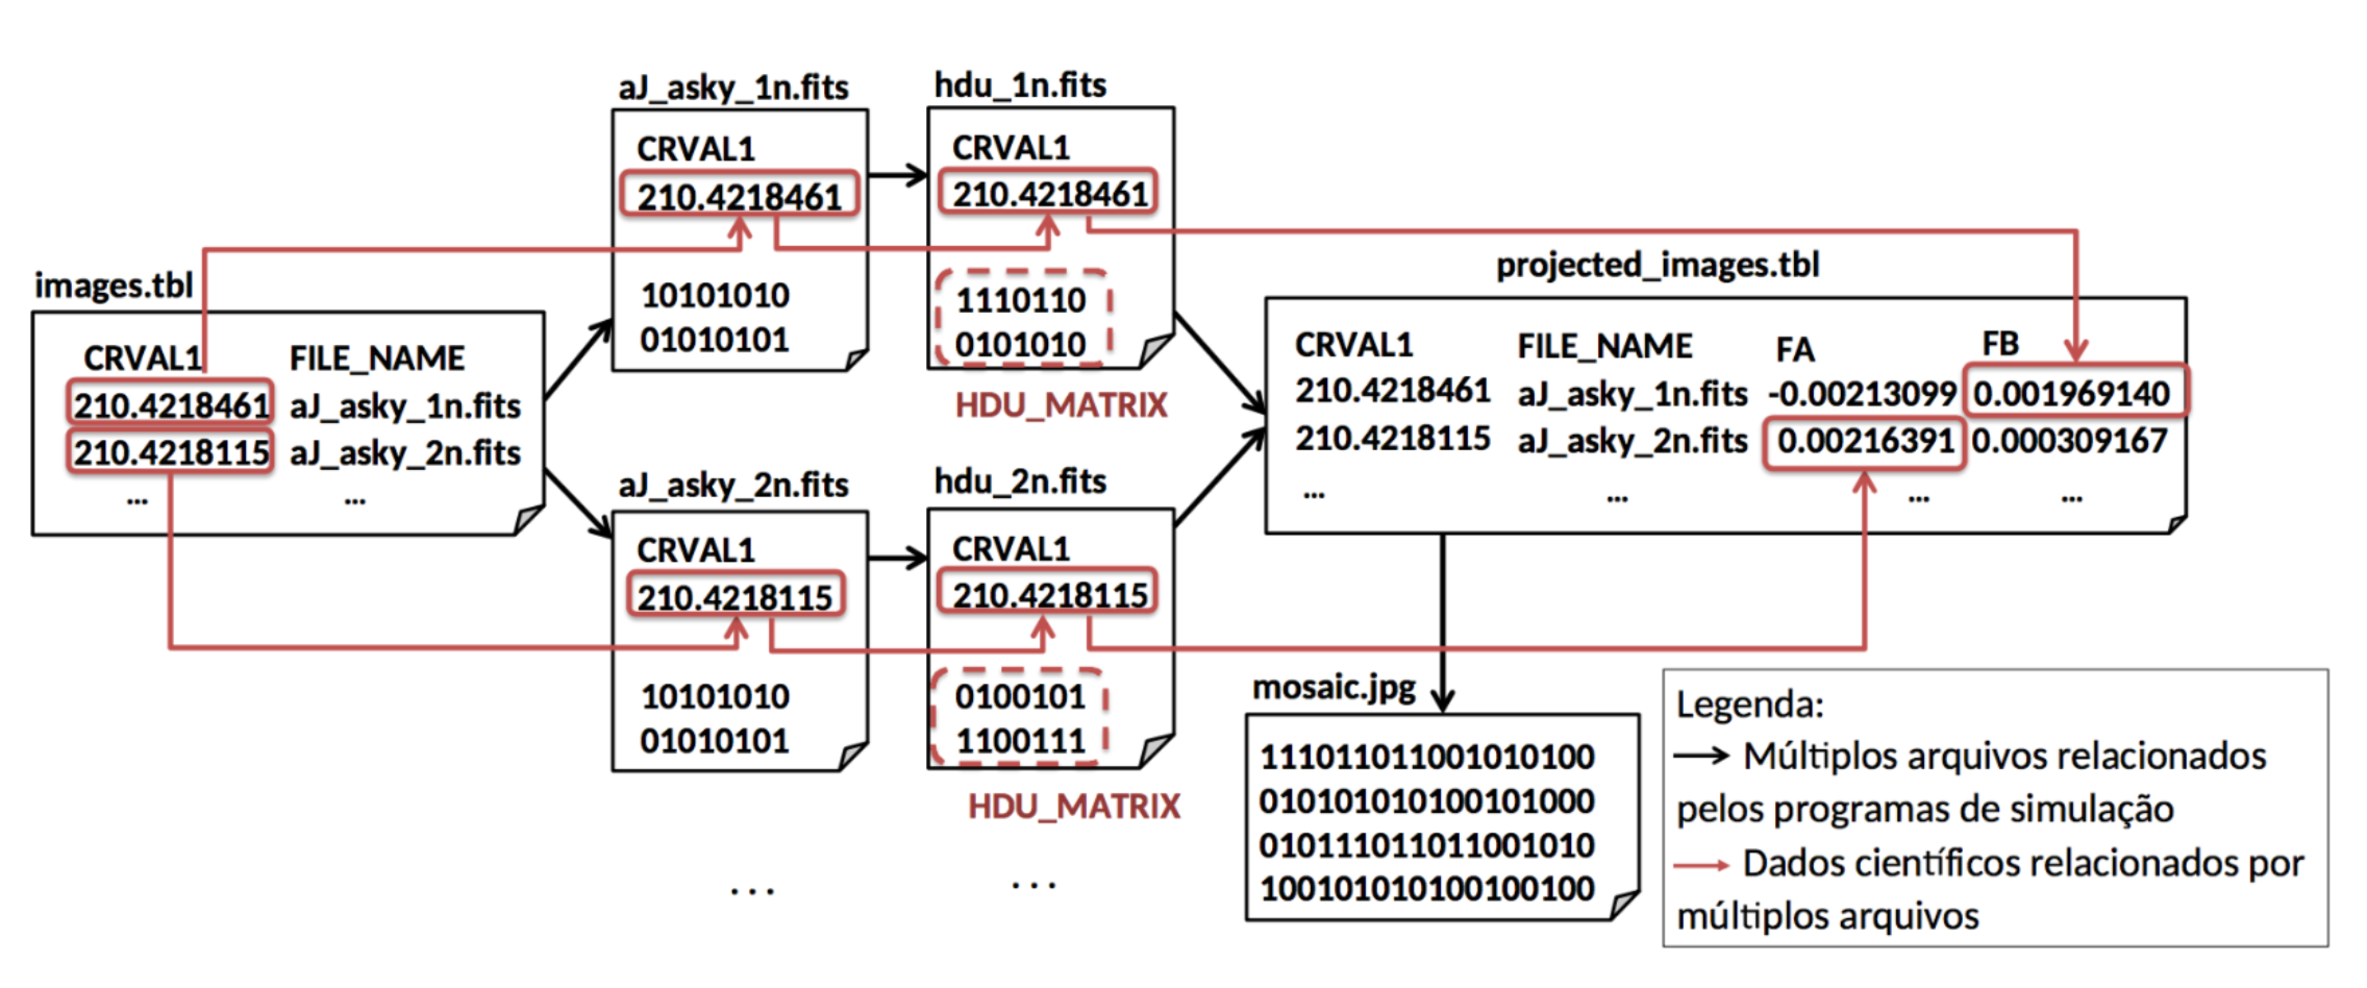
\includegraphics[width=\textwidth]{img/types-of-queries-1-2-3}
    \caption[Exemplo de análise de uma simulação de astronomia]{Exemplo de uma simulação de astronomia para análise de arquivos de dados científicos. Encontrada originalmente em~\cite{silva2015propostadoutorado}.}%
    \label{fig:types-of-queries-1-2-3}
\end{figure}

\section{Análise de dados científicos isolados}%
\label{sec:analise-de-dados-cientificos-isolados}

Consultas do \textbf{tipo 1} são caracterizadas pela \textbf{análise} (do inglês: \textit{parsing}) \textbf{de dados científicos}, encontrados em arquivos que foram produtos de uma simulação computacional, e envolve tipicamente a \textbf{extração} ou \textbf{interpretação} desses dados de acordo com o domínio da aplicação da simulação. É necessário conhecer a estruturação e~/~ou a codificação utilizada nesses arquivos para que seja possível acessá-los e extrair um significado semântico dos dados do mesmo; além disso, cada formato de arquivo possui programas específicos e peculiares para a sua análise e extração: por exemplo, um arquivo em formato de imagem tal como o \abbrev{PNG}{\textit{Portable Network Graphics}} PNG (Portable Network Graphics) pode ser analisado (visualizado) por um editor de imagens, enquanto que um arquivo em formato de música tal como o \abbrev{WAV}{Waveform Audio File Format} WAV (\textit{Waveform Audio File Format}) pode ser analisado (reproduzido) por um \textit{player} de áudio. Em particular, destaca-se que a semântica da análise --- reprodução, visualização, extração, etc --- é inerente ao tipo de arquivo analisado.

Esses dados e seus respectivos arquivos podem estar ou não em formato binário; por exemplo, um arquivo em formato \abbrev{JSON}{JavaScript Object Notation} JSON (JavaScript Object Notation) geralmente contém dados em formato de texto; enquanto que um arquivo FITS (Flexible Image Transport System)~\cite{greisen2002representations}, utilizado em astronomia, pode possuir parte de seus dados em formato binário assim como o NetCDF (Network Common Data Form)~\cite{rew1990netcdf}, utilizado em dinâmica de fluidos computacionais.

Consultas do tipo 1 são as mais simples de serem realizadas em relação às outras. Em primeiro lugar, elas são auto-contidas no que diz respeito aos dados científicos, isto é, apenas a presença desses dados é suficiente para que esse tipo de consulta possa ser realizado: não é necessária a especificação sobre o fluxo de dados da simulação computacional. Em segundo lugar,

\perrotta{TODO}

\perrotta{Técnicas de indexação --> FastBit, NoDB, RAW}

\section{Rastreio de fluxos de arquivos}%
\label{sec:rastreio-de-fluxos-de-arquivos}
\perrotta{Capítulo 03 --- Soluções para análise do fluxo de arquivos (citar sistemas existentes: Chiron; Pegasus; Kepler; etc)}

\perrotta{sistema de workflows --> gerência do fluxo de arquivos}

\section{Rastreio de fluxo de elementos de dados em múltiplos arquivos}%
\label{sec:rastreio-de-elemento-de-dados-em-multiplos-arquivos}
\perrotta{Capítulo 03 --- Soluções para análise do fluxo de elementos de dados relacionados em múltiplos arquivos
DfAnalyzer (grupo)
YesWorkflow
NoWorkflow
CCPE (mais sistemas)
}